\section{Transformer} \label{sec:Transformer}
% 
% \begin{figure}[h]
% \vspace{-10pt}
% \centering
% 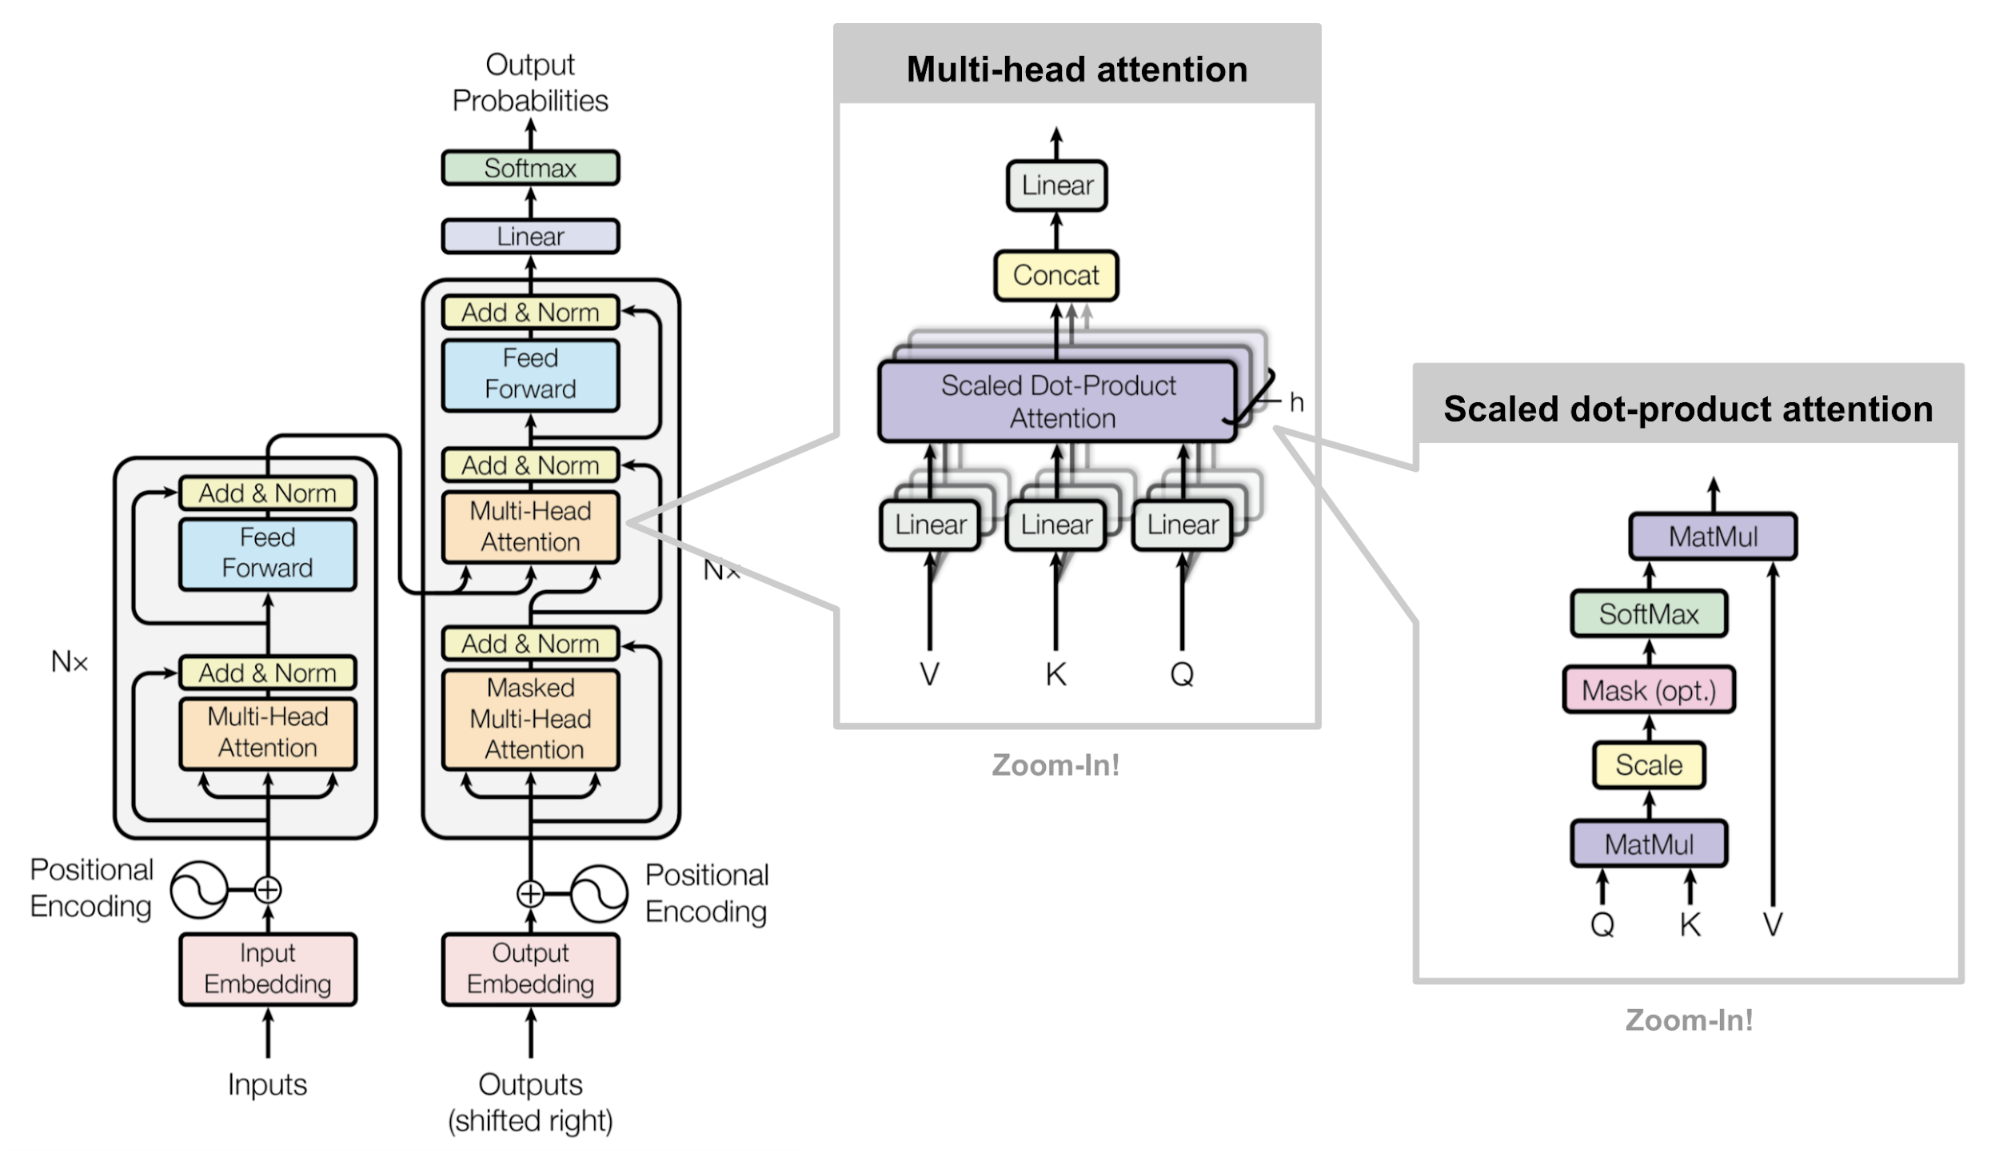
\includegraphics[width=0.95\textwidth]{imgs/transformer.png}
% \vspace{-10pt}
% \caption{Transformer model architecture. The gray boxes hold Encoder and Decoder layers, respectively, which are each repeated $N=6$ times. From \emph{Attention? Attention}, by Weng, 2018. \url{https://lilianweng.github.io/lil-log/2018/06/24/attention-attention.html}. Copyright 2018 by Weng.}
% \vspace{-5pt}
% \label{fig:transformer}
% \end{figure}

The \textbf{Transformer model} introduced by Vaswani et al. (2017) for \nameref{nlptask:neuralmachinetranslationNMT} proves more parallelizable than general seq-to-seq models with attention. Rather than \hyperref[sec:RNN]{ recurrent neural networks (RNNs)} combined with the \textbf{\hyperref[sec:AttentionMechanism]{attention mechanism}}, the Transformer \hyperref[sec:Seq2Seq]{sequence-to-sequence model} is composed of only a \textbf{\hyperref[sec:SelfAttention]{self attention mechanism}} to attend to different input tokens for generating a sequence of \hyperref[sec:SolutionWithContextEmbs]{contextual embeddings}. 
%It is illustrated in \cref{fig:transformer}.




\subsection{Self-Attention} \label{sec:SelfAttention}

\subsubsection{Motivation for Self-Attention}

{\large ``}\textit{The animal didn't cross the road because it was too tired.}{\large "}

%\begin{shadequote}{}
%\vspace{10pt}
%\large \textit{The animal didn't cross the road because it %was too tired.}
%\vspace{10pt}
%\end{shadequote}

What does ``it” in this sentence refer to? Is ``it" referring to the road or to the animal? This question may be simple to a human but not to a machine.  

This is the motivation for using \textbf{self-attention}: when the Transformer processes the word ``it", self-attention allows it to associate ``it" with ``animal". As the Transformer processes each word, self-attention allows it to look at other positions in the input sentence for clues on creating a better encoding for this word. In each layer, a part of the attention mechanism that focuses on ``the animal" was \emph{baked in} to a part of the representation of the word ``it" (Trevett, 2020). 


\subsubsection{Query, Key, Value} \label{sec:QKV}

Formally, ``an \textbf{\textit{attention function}} can be described as mapping a query and a set of key-value vectors pairs to an output. (Vaswani et al., 2017). The \textbf{Query matrix $Q$} contains row-wise information for which word to calculate self attention; the \textbf{Key matrix $K$} holds word vector representations on its rows, for \emph{each} word in the sentence, and the \textbf{Value matrix $V$} contains vector row-wise information for the rest of the words in the sentence. Multiplying the query vector with the key vector of a particular word, stored in $Q$ and $K$ computes a result that indicates how much \emph{value} vector $V$ to consider.

For above example sentence, $Q$ refers to ``it"; $V$ has vectors for words other than ``it", and $K$ has vectors for each word, including ``it".  The final calculated word embedding or \textbf{output} is a weighted sum of \textbf{value} vectors and \hyperref[cnc:softmaxLayer]{softmax probabilities} of the dot product between query and key vectors, as in \cref{eq:SelfAttention}:

\vspace{-5pt}

\begin{equation}
\texttt{Attention} \Big(Q, K, V \Big) = \texttt{softmax} \Bigg(\frac {QK^T} {\sqrt{d_k}} \Bigg) V
\label{eq:SelfAttention}
\end{equation}

\nameref{app:TransformerSelfAttnCalc} describes in complete detail the vector and matrix version calculations of self attention. 


\subsection{Multi-Head Attention} \label{sec:MultiHeadAttention}

\subsubsection{Motivation for Multi-Head Attention}


%A single attention head cannot do this because of averaging (Vaswani et al., 2017).  

A \textbf{multi-head attention mechanism} comprises of several self-attention heads, enabling the Transformer to ``jointly attend to information from different representation subspaces at different positions." Instead of calculating attention once, multi-head attention does self attention many times in parallel on the projected dimensions, concatenates the independent attention outputs, and once again projects the result into the expected dimension to give a final value (Vaswani et al., 2017; Weng, 2018).  

%``linearly projects the queries, keys and values $H$ (number of attention heads) times with different, learned linear projections to $d_k$, $d_k$, and $d_v$ dimensions, respectively." 

In the example sentence, when the Transformer encodes the word ``it," one attention head may focus most on ``the animal" while another head focuses on ``tired", so the Transformer's ``it" vector incorporates some representation of all the words in the sentence (Trevett, 2020). 

\subsubsection{Multi-Head Attention: Matrix Calculation}

Using notation from Vaswani et al. (2017) and Alammar (2018b): 

\begin{enumerateSpaced}{3pt}
    \item \textbf{Create $Q$, $K$, $V$ matrices}: With multi-headed attention there are now separate $Q$, $K$, $V$ weight matrices for each attention head $h$, in $1 \leq h \leq H$. Each row of input matrix $X$ corresponds to a word in the input sentence. For each attention head, $X$ is multiplied by trained parameter matrices to produce the separate query, key, value matrices: 
    \begin{center}
    \begin{tabular}{ c  c  c }
    $Q_h = X \cdot W_h^Q$
    &
    $K_h = X \cdot W_h^K $
    &
    $V_h = X \cdot W_h^V $
    \end{tabular}
    \end{center}\label{eq:QKVMultihead}

    where $H =$ number of attention heads, and the dimensions of the parameter matrices are $\large W_h^Q \in \mathbb{R}^{\Large d_{model} \times d_k}$, $\large W_h^K \in \mathbb{R}^{\Large d_{model} \times d_k}$, and $\large W_h^V \in \mathbb{R}^{\Large d_{model} \times d_v}$. 
    
    \item \textbf{Apply Softmax To Get Output Matrix}: Steps two through six in the \hyperref[app:TransformerSelfAttnCalc]{vector calculation of self-attention} can be condensed in a single matrix step to find the final output matrix $Z_h$ for the $h$-th attention head for any self-attention layer:
    \begin{equation}
    Z_h := \texttt{softmax} \Bigg(\frac {Q_h K_h^T} {\sqrt{d_k}} \Bigg) \cdot V_h
    \label{eq:ZMultihead}
    \end{equation}
    
    \item \textbf{Concatenate Output Matrices}: Now there are $H$ different output matrices $Z$ for each attention head. But the feed-forward layer is only expecting a single matrix instead of $H$. So, this step concatenates the $H$ matrices and multiplies the result by an additional weights matrix $W^O$ to return to expected dimensions. 
    \begin{equation}
    \texttt{MultiHeadAttention}(Q, K, V) = \texttt{Concat}(\texttt{head}_1, ..., \texttt{head}_H) \cdot W^O
    \label{eq:MultiheadAttention}
    \end{equation}
      where $\texttt{head}_i = \texttt{Attention}(Q \cdot W_h^Q, K \cdot W_h^K, V \cdot W_h^V)$, where $\texttt{Attention}(Q, K, V) = \texttt{softmax} \Bigg( \frac {\Large QK^T} {\Large \sqrt{d_k}} \Bigg) \cdot V$ as before and  $W^O \in \mathbb{R}^{\Large H \cdot d_v \times d_{model}}$.
    
    
\end{enumerateSpaced}



\subsection{Positional Encodings} \label{sec:PosEncodings}

\subsubsection{Motivation for Positional Encodings}

Since the Transformer contains no recurrence mechanism it does not benefit from its resulting way of seeing order in the input sequence sentence. Instead, Vaswani et al. (2017) use \textbf{positional encodings} to inject absolute positional information of tokens into the sequence. Otherwise, the sentences ``I like dogs more than cats" and ``I like cats more than dogs" incorrectly would encode the same meaning (Raviraja, 2019). 

A \textbf{positional encoding} follows a specific, learned pattern to identify word position or the distance between words in the sequence (Alammar, 2018b). They use sinusoidal waves to attend to relative positions since for any fixed offset $k$, the positional encoding $\texttt{PosEnc}_{\texttt{pos} + k}$ can be represented as a linear function of $\texttt{PosEnc}_{\texttt{pos}}$.

\vspace{-10pt}

\begin{center}
\begin{tabular}{ c  c }
$
\begin{array}{ll}
\texttt{PosEnc}_{\Large (\texttt{pos}, 2i)} = \text{sin} \Bigg(\frac {\texttt{pos}} {10000^{\Large \frac {2i} {d_{\texttt{model}}} } }  \Bigg)
\end{array}
$
&
$
\begin{array}{ll}
\texttt{PosEnc}_{\Large (\texttt{pos}, 2i + 1)} = \text{cos} \Bigg(\frac {\texttt{pos}} {10000^{\Large \frac {2i} {d_{\texttt{model}}} } }  \Bigg)
\end{array}
$
\end{tabular}
\end{center}

%where $\texttt{pos} = $ a position, $i = $ a dimension.


\subsection{Position-wise Feed Forward Layer} \label{sec:PositionwiseFFNLayers}

A \textbf{positionwise feed-forward layer} is a kind of \hyperref[sec:NeuralNetRepr]{feed-forward neural network (FNN)} applied to each position separately and identically. The FFN contains two linear transformations with a $\texttt{ReLU}$ or $\texttt{max}$ activation function between them: $\texttt{FFN}(x) = \texttt{ReLU}(0, x W_1 + b_1) W_2 + b_2$



\subsection{Residual Connection} \label{sec:ResidualConnections}

A \textbf{residual connection} is a sub-layer in both Encoder and Decoder stacks which adds inputs to outputs of a sub-layer. This allows gradients during optimization to directly flow through a network rather than undergo transformation by nonlinear activations $\texttt{LayerNorm}(x + \texttt{Sublayer}(x))$, where $\texttt{Sublayer}(x)$ is a general function representing the sub-layer's operation. Each sub-layer in the stack, such as \hyperref[sec:SelfAttention]{self-attention} and \hyperref[sec:PositionwiseFFNLayers]{positionwise feed forward layer}s, are surrounded by residual connection layers followed by layer normalization (Raviraja, 2019). 




\subsection{Masked Multi-Head Attention} \label{sec:MaskedMultiHeadAttention}

The Decoder uses a sub-layer called \textbf{masked self attention}, which is an \hyperref[sec:AttentionMechanism]{attention mechanism} with \textbf{masking} to prevent positions from attending to subsequent positions. With masking, when the Decoder decodes embedding $\overrightarrow{w_i}$, it becomes unaware of words  $\overrightarrow{w_{>i}}$ past position $i$ and thus can only use words $\overrightarrow{w_{\leq i}}$. This protects the Transformer from cheating on predictions (Ta-Chun, 2018). 

\subsection{Encoder-Decoder Attention} \label{sec:EncoderDecoderAttention}

This \textbf{encoder-decoder \hyperref[sec:AttentionMechanism]{attention layer}} is similar to \hyperref[sec:MultiHeadAttention]{multi-head self attention} but it creates the query matrix $Q$ from the layer below it (a Decoder self attention layer) and uses the key $K$ and value $V$ matrices from the Encoder stack's output (Alammar, 2018b). 



\subsection{Encoder} \label{sec:TransformerEncoder}

The Encoder is a \textbf{\hyperref[sec:BidirectionalLM]{bidirectional} \hyperref[sec:RNN]{recurrent network (RNN)}}. The \hyperref[sec:ForwardLM]{forward} \hyperref[sec:RNN]{RNN} reads the input sequence $\overrightarrow{x} = \Big\{ x_1,...,x_{T_x} \Big\}$ from left to right to produce a sequence of forward hidden states $\Big\{ \overrightarrow{h_1},..., \overrightarrow{h_{T_x}} \Big\}$. The \hyperref[sec:BackwardLM]{backward} RNN reads the sequence in reverse order and returns a sequence of backward hidden states $\Big\{ \overleftarrow{h_1},..., \overleftarrow{h_{T_x}} \Big\}$. Then, for each word $x_t$ an annotation is obtained by concatenating the corresponding forward hidden state vector $\overrightarrow{h}_t$ with the backward one $\overleftarrow{h}_t$, such that $h_t = \Big \{ \overrightarrow{h}_t^T \; ; \; \overleftarrow{h}_t^T \Big\}^T , \: t=1,...,T_x$. (Note: arrows here denote the direction of the network rather than vector notation.) This allows the annotation vector $h_t$ for word $x_t$ to contain bidirectional context (Bahdanau et al., 2016). 

The Encoder is composed of $N$ identical \textbf{Encoder layers}, which together are named the \textbf{Encoder stack}. A single \textbf{Encoder layer} is composed of the sub-layers \textbf{\nameref{sec:MultiHeadAttention}} and \textbf{ \nameref{sec:PositionwiseFFNLayers}} (Trevett, 2020). 

%A \hyperref[sec:ResidualConnections]{residual connection layer} surrounds each of these sub-layers, and is followed by \textbf{layer normalization} (Trevett, 2020).  




\begin{figure}[h]
\vspace{-5pt}
\centering
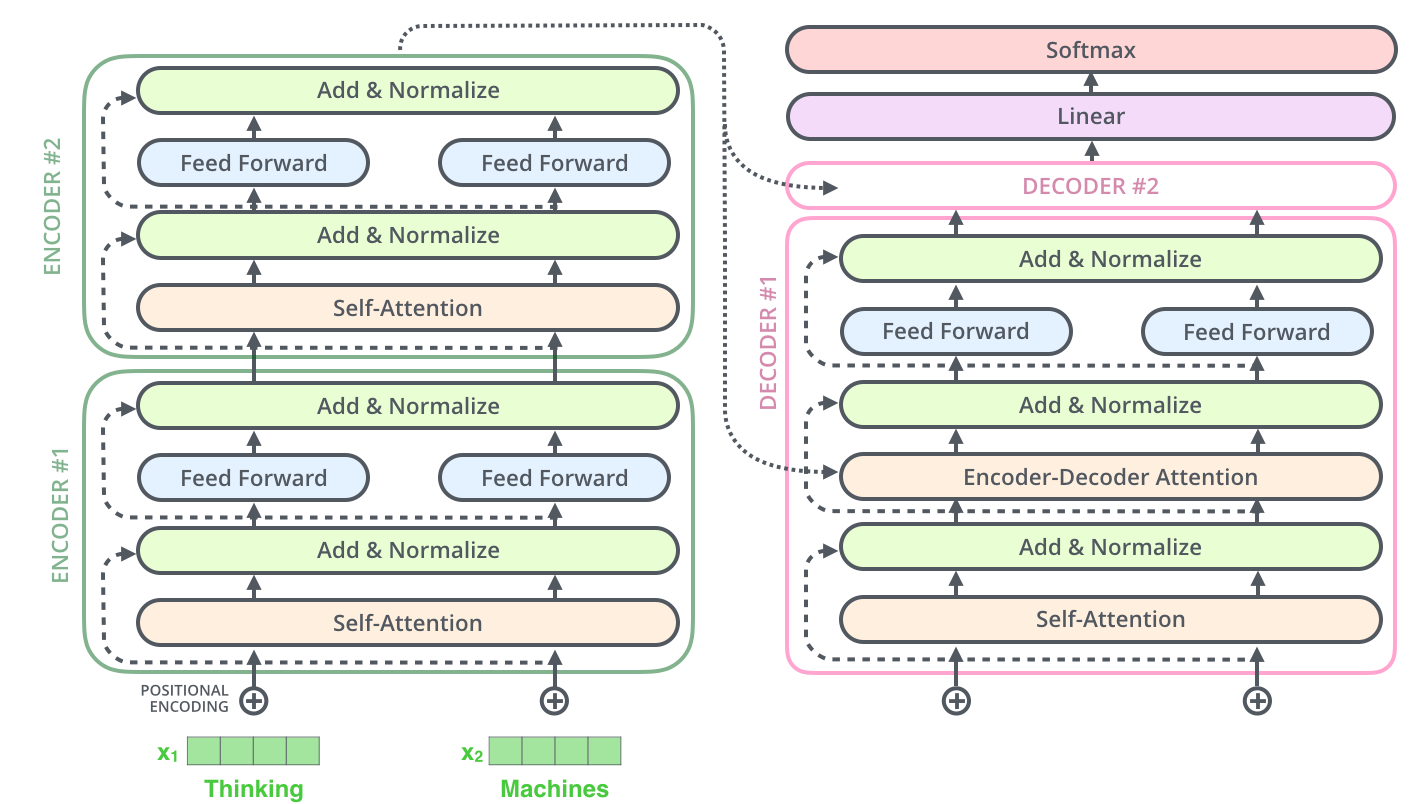
\includegraphics[width=0.8\textwidth]{imgs/encoderDecoderLayersDetailed.png}
\vspace{-5pt}
\caption{ The layers inside Encoder and Decoder. From \emph{The Illustrated Transformer}, by Alammar, 2018. \url{https://jalammar.github.io/illustrated-transformer/}. Copyright 2018 by Alammar.}
\vspace{-5pt}
\label{fig:encDecLayersDetailed}
\end{figure}




\subsection{Decoder} \label{sec:TransformerDecoder}


The Decoder \hyperref[sec:NeuralLM]{neural network} generates hidden states $s_t = \text{Decoder}\Big( s_{t-1}, y_{t-1}, c_t \Big)$ for time steps $t = 1,..., m$ where the context vector $c_t = \sum_{i=1}^n \alpha_{ti} \cdot h_i$ is a sum of the hidden states of the input sentence, weighted by alignment scores, as for the \hyperref[sec:Seq2Seq]{Seq-to-Seq} model (Weng, 2018). 

Similarly to the Encoder, the Decoder contains a stack of $N$ Decoder layers, each of which consists of three sub-layers: \textbf{\nameref{sec:MaskedMultiHeadAttention}}, and \textbf{\nameref{sec:EncoderDecoderAttention}}, and lastly \textbf{ \nameref{sec:PositionwiseFFNLayers}}. 

%Like in the Encoder, in between each of these layers is a \hyperref[sec:ResidualConnections]{residual connection} followed by layer normalization. The Encoder and Decoder stack are shown in \cref{fig:encDecLayersDetailed}. 




\subsection{Final Linear and Softmax Layer} \label{sec:TransformerFinalLayer}


The Decoder stack outputs a vector of floats. Then, the \textbf{Linear Layer}, a \hyperref[sec:NeuralLM]{fully-connected neural network}, projects the Decoder's output vector in a larger-dimensioned ``logits vector" so each cell holds a score corresponding to each unique vocabulary word. After, a \textbf{Softmax Layer} then converts the Linear Layer's scores into probabilities using \hyperref[cnc:softmaxLayer]{softmax function}. To find the predicted word, the cell with highest probability is chosen, and corresponding word is called the predicted word, and is output for a particular time step.



% 
% \subsection{Transformer Workflow} \label{sec:TransformerWorkflow}
% 
% Alammar (2018b) describes the procedure governing the Transformer's moving parts as follows: 
% 
% \begin{enumerateSpaced}{3pt}
%     \item The \nameref{sec:TransformerEncoder} processes the input sentence in the given language, adding the \hyperref[sec:PosEncodings]{positional encoding} to input embeddings.
%     
%     \item The output of the top \nameref{sec:TransformerEncoder} layer is then transformed into a set of \hyperref[sec:AttentionMechanism]{attention} vectors $K$ and $V$.
%     
%     \item The \nameref{sec:TransformerDecoder} uses $K$ and $V$ in its \hyperref[sec:EncoderDecoderAttention]{encoder-decoder attention layer} to help the \nameref{sec:TransformerDecoder} focus on appropriate places in the input sequence. Subsequent outputs are fed to the bottom \nameref{sec:TransformerDecoder}, allowing \nameref{sec:TransformerDecoder}s to accumulate results. Also, the \nameref{sec:TransformerDecoder} includes \hyperref[sec:PosEncodings]{positional encoding}s to its inputs. 
%     
%     \item The previous steps are repeated until a special symbol is reached, indicated the \nameref{sec:TransformerDecoder} has finished generating output.
%     
%     \item The \nameref{sec:TransformerDecoder}'s numeric output vector is passed through the \hyperref[sec:TransformerFinalLayer]{final linear and softmax layer} to find a predicted, translated word in the target language. 
%     
% \end{enumerateSpaced}

